\chapter{Potenzreihen und elementare Funktionen}
\begin{fdefinition}[Potenzreihe]
%MARK: Definition 2.14
Die (formale) Reihe $\sum_{n = 0}^{\infty} a_n (x - x_0)^n$ hei�t \indexb{Potenzreihe} mit Entwicklungspunkt $x_0$ und Koeffizienten $(A_n)_{n \in \N_0}$
\end{fdefinition}

\begin{bemerkung}
Man setzt $0^0 = 1$
\end{bemerkung}

\begin{fsatz}
\label{satz:Potenzreihen_und_elementare_Funktionen_S2_15}
F�r die Potenzreihe $\sum_{n = 0}^{\infty} a_n (x - x_0)^n$ gilt:
\begin{enumerate}[label=\roman*)]
\item konvergiert die Reihe $a_n$ einer Stelle $x_1 \neq x_0$, so konvergiert sie f�r alle $x$ mit $\betrag{x - x_0} < \betrag{x_1 - x_0}$
\item divergiert die Reihe $a_n$ einer STelle $x_2 \neq x_0$, so divergiert sie f�r alle $x$ mit $\betrag{x - x_0} > \betrag{x_2 - x_0}$
\end{enumerate}
\Mark{Satz 2.15}
\end{fsatz}

\begin{fbeweis}
\mbox{}\par
\begin{enumerate}[label=\roman*)]
\item $\sum_{n = 0}^{\infty} a_n (x_1 - x_0)^n$ konvergent \Ra $\lim_{n \ra \infty} a_n (x_1 - x_0)^n = 0$
		\begin{align*}
		&\sum_{n = 0}^{\infty} a_n (x - x_0)^n\\
		\Lra & \forall \epsilon > 0 \exists N(\epsilon) \forall k \grgl N(\epsilon)\\
		&\betrag{a_n(x_1 - x_0)^n} < \epsilon\\
		\Ra & \sum_{n = 0}^{\infty} \betrag{a_n (x - x_0)^n} = \sum_{n = 0}^{N - 1} \betrag{a_n (x - x_0)^n} + \sum_{n = N}^{\infty} \betrag{_n (x - x_0)^n}\\
		= & \sum_{n = 0}^{N - 1} \underbrace{\betrag{a_n (x - x_0)^n}}_{\tx{endlich}} + \sum_{n = N}^{\infty} \betrag{\underbrace{a_n (x_1 - x_0)^n}_{< \epsilon}} \betrag{\underbrace{\rklamm{\frac{x - x_0}{x_1 - x_0}}^n}_{< 1}}\\
		= & \underbrace{\sum_{n = 0}^{N - 1} \betrag{a_n (x - x_0)}}_{\tx{endlich}} + \epsilon \underbrace{\sum_{n = N}^{\infty} \betrag{\underbrace{\frac{x - x_0}{x_1 - x_0}}_{= q < 1}}^n}_{\begin{minipage}{2cm}\begin{center}\scriptsize{konvergente geometrische Reihe}\end{center}\end{minipage}} \Ra \tx{ konvergent}
		\end{align*}

\item Widerspruchsbeweis
		\[\sum_{n = 0}^{\infty} a_n (x_2 - x_0)^n \tx{ divergent}\]
		Annahme: $\exists x_3$ mit $\betrag{x_3 - x_0} > \betrag{x_2 - x_0}$
		\[\sum_{n = 0}^{\infty} a_n (x_3 - x_0)^n \tx{ konvergent}\]
		\stack{i)}{\Ra} $\sum_{n = 0}^{\infty} a_n (x_2 - x_0)^n$ konvergent \blitza
\end{enumerate}
\end{fbeweis}

\begin{fsatz}[Konvergenzradius einer Potenzreihe]
F�r jede Potenzreihe $\sum_{n = 0}^{\infty} a_n (x - x_0)^n$ existiert ein eindeutig bestimmter \indexb{Konvergenzradius} $r$ ($0 \klgl r \klgl \infty$) f�r den gilt:
\begin{enumerate}
\item Falls $r = 0$ so konvergiert die Potenzreihe nur f�r $x = x_0$
\item Falls $0 < r < \infty$ so konvergiert die Potenzreihe f�r alle $x \in \mb{R}$ mit $\betrag{x - x_0} < r$ und divergiert f�r alle $x \in \mb{R}$ mit $\betrag{x - x_0} > r$.
\item Falls $r = \infty$, so konvergiert die Potenzreihe f�r alle $x \in \mb{R}$
\end{enumerate}
\Mark{Satz 2.16}
\end{fsatz}

\begin{fbeweis}
Folgt aus Satz \vref{satz:Potenzreihen_und_elementare_Funktionen_S2_15}.
\Solved{Insert ref to Satz 2.15}{}
\end{fbeweis}

\begin{fdefinition}[Konvergenzbereich]
%MARK: Definition 2.17
Der \indexb{Konvergenzbereich} einer Potenzreihe $\sum_{n = 0}^{\infty} a_n (x - x_0)^n$ ist $K = \gklamm{x \in \mb{R} \vert \sum_{n = 0}^{\infty} a_n (x - x_0)^n \tx{ konvergent}}$. Es gilt:
\[(x_0 - r, x_0 + r) \subseteq K \subseteq \eklamm{x_0 - r, x_0 + r}\]
\end{fdefinition}

\begin{beispiel}
geometrische Reihe $\sum_{n = 0}^{\infty} (x - x_0)^n$
\begin{itemize}[label=\Ra]
\item Konvergenzradius $r = 1$
\item $(x_0 - 1, x_0 + 1) \subseteq K \subseteq \eklamm{x_0 - 1, x_0 + 1}$
		\begin{description}
		\item[$x = x_0 - 1$] $\sum_{n = 0}^{\infty} \rklamm{\rklamm{x_0 - 1} - x_0}^n = \sum_{n = 0}^{\infty} (-1)^n$ divergent
		\item[$x = x_0 + 1$] $\sum_{n = 0}^{\infty} \rklamm{\rklamm{x_0 + 1} - x_0}^n = \sum_{n = 0}^{\infty} 1^n$ divergent
		\end{description}
\item $K = (x_0 -1, x_0 + 1)$
\end{itemize}
\end{beispiel}

\begin{fsatz}[Bestimmung des Konvergenzradius]
%MARK: Satz 2.18
Sei $\sum_{n = 0}^{\infty} a_n (x - x_0)^n$ gegeben
\begin{enumerate}[label=\roman*)]
\item Existiert $q = \lim_{n \ra \infty} \betrag{\frac{a_n}{a_{n + 1}}}$, so ist der Konvergenzradius $r = q$
\item Existiert $w = \lim_{n \ra \infty} \sqrt[n]{\betrag{a_n}}$, so ist der Konvergenzradius $r = \frac{1}{w}$\\
		Wobei "`$\frac{1}{0}$"'$ = \infty$ und "`$\frac{1}{\infty}$"'$ = 0$
\end{enumerate}
\end{fsatz}

\begin{fbeweis}
Anwendung des Quotienten \ac{bzw.} Wurzelkriteriums auf die Reiher $\sum_{n = 0}^{\infty} A_n$ mit
\[A_n = a_n (x - x_0)^n\]
\end{fbeweis}

\begin{beispiel}
\mbox{}\par
\begin{enumerate}
\item $\sum_{n = 0}^{\infty} \frac{x^n}{n!} = \sum_{n = 0}^{\infty} \ub{\frac{1}{n!}}{= a_n} \mal \rkl{x - \ub{0}{= x_0}}^n$\\
		Entwicklungspunkt $x_0 = 0$\\
		Quotientenmethode
		\begin{align*}
		\lim_{n \ra \infty} \betrag{\frac{a_n}{a_{n + 1}}} &= \lim_{n \ra \infty} \betrag{\frac{1}{n!} \mal \frac{(n + 1)!}{1}} = \lim_{n \ra \infty} \frac{(n + 1)!}{n!}\\
		&\lim_{n \ra \infty} (n + 1) = \infty
		\end{align*}
		\begin{itemize}[label=\Ra]
		\item Konvergenzradius $r = q = \infty$
		\item Konvergenzbereich $K = \mb{R}$
		\end{itemize}

\item $\sum_{n = 0}^{\infty} \frac{1}{2^n} x^n = \sum_{n = 0}^{\infty} \ub{\frac{1}{2^n}}{= a_n} \rkl{x - \ub{0}{= x_0}}^n$\\
		Entwicklungspunkt $x_0 = 0$\\
		Wurzelmethode
		\[w = \lim_{n \ra \infty} \sqrt[n]{\betrag{a_n}} = \lim_{n \ra \infty} \sqrt[n]{\betrag{\frac{1}{2^n}}} = \lim_{n \ra \infty} \frac{1}{2} = \frac{1}{2}\]
		\begin{itemize}[label=\Ra]
		\item Konvergenzradius $r = \frac{1}{w} = 2$\\
				$(-2, 2) \subseteq K \subseteq \eklamm{-2 , 2}$
				\begin{description}
				\item[$x = -2$] $\sum_{n = 0}^{\infty} \frac{1}{2^n} (-2)^n = \sum_{n = 0}^{\infty} (-1)^n$ divergent
				\item[$x = 2$] $\sum_{n = 0}^{\infty} \frac{1}{2^n} (2)^n = \sum_{n = 0}^{\infty} 1^n$ divergent
				\end{description}

		\item $K = (-2, 2)$
		\end{itemize}

\item $\sum_{n = 0}^{\infty} n^n (x + 2)^n = \sum_{n = 0}^{\infty} \ub{n^n}{a_n} \rkl{x - \ub{(-2)}{= x_0}}^n$\\
		Entwicklungspunkt $x_0 = -2$
		Wurzelmethode
		\[w = \lim_{n \ra \infty} \sqrt[n]{\betrag{a_n}} = \lim_{n \ra \infty} \sqrt[n]{n^n} \lim_{n \ra \infty} n = \infty\]
		\begin{itemize}[label=\Ra]
		\item Konvergenzradius $r = \frac{1}{w} = 0$
		\item $K =\gklamm{-2}$
		\end{itemize}
\end{enumerate}
\end{beispiel}

\section{Aufgabe 2.5}
\label{sec:Potenzreihen_und_elementare_Funktionen_A2_5}
Bestimmen Sie den Entwicklungspunkt, den Konvergenzradius und den Konvergenzbereich der folgenden Potenzreihen.
\begin{enumerate}[label=\alph*)]
\item $\sum_{n = 0}^{\infty} 3n (x + 1)^n$
\item $\sum_{n = 0}^{\infty} \frac{1}{n^n} \mal x^n$
\item $\sum_{k = 0}^{\infty} \frac{(2x + 1)^k}{k + 3}$
\end{enumerate}

L�sung siehe \vref{sec:Potenzreihen_und_elementare_Funktionen_A2_5L}.

\begin{bemerkung}
Die Potenzreihe $\sum_{n = 0}^{\infty} a_n \mal (x - x_0)^n$ definiert in ihrem Konvergenzbereich eine Funktion
\begin{align*}
f: &K \ra \mb{R}\\
&x \mapsto f(x) = \sum_{n = 0}^{\infty} a_n \mal (x - x_0)^n
\end{align*}
Auf diese Weise kann man einige elementare Funktionen definieren. Zum Beispiel Exponentialfunktion, Sinus, Cosinus.
\end{bemerkung}

\begin{fdefinition}[Exponentialfunktion]
%MARK: Definition 2.20
Die Funktion
\begin{align*}
\exp: \mb{R}& \ra \mb{R}\\
x& \mapsto \exp (x) = \sum_{n = 0}^{\infty} \frac{1}{n!} \mal x^n = e^x
\end{align*}
hei�t Exponentialfunktion

\begin{center}
\begin{tikzpicture}[domain=-2.5:1.2]
\draw[->,thick] (-2.5,0) -- (4.5,0) node[below] {$x$};
\draw[->,thick] (0,-0.5) -- (0,3.5);
\node at (0,0) [below right] {$0$};
\draw[thick] (-0.05,1) -- (0.05,1) node[left] {$1$};

\foreach \x in {1,2,3,4}
	\draw[thick] (\x,-0.05) -- (\x,0.05);

\draw plot[smooth] (\x,{exp(\x)}) node[right] {$\exp (x)$};
\end{tikzpicture}
\end{center}
\Img{MA-16.04.2009-IMG-1}

\end{fdefinition}

\begin{fsatz}[Eigenschaften der Exponentialfunktion]
%MARK: Satz 2.21
\mbox{}\par
\begin{enumerate}[label=\roman*)]
\item $\forall x, y \in \mb{R}$: $e^x \mal e^y = e^{x + y}$ Funktionalgleichung
\item $e^0 = 1$, $e^1 = e$, $e^{-x} = \frac{1}{e^x}$
\item $x < 0$: $0 < e^x < 1$\\
		$x > 0$: $e^x > 1$

\item $\lim_{x \ra -\infty} e^x = 0$, $\lim_{x \ra \infty} e^x = \infty$\\
		$\forall n \in \N$: $\lim_{x \ra \infty} \frac{x^n}{e^x} = 0$
\end{enumerate}
\end{fsatz}

\begin{fbeweis}
\mbox{}\par
\begin{enumerate}[label=\roman*)]
\item $e^x \mal e^y$
		\[e^x \mal e^y = \rkl{\sum_{n = 0}^{\infty} \ub{\frac{x^n}{x!}}{= A_n}} \mal \rkl{\sum_{n = 0}^{\infty} \ub{\frac{y^n}{n!}}{= B_n}} = \sum_{n = 0}^{\infty} C_n\]
		\begin{align*}
		C_n &= \sum_{l = 0}^{n} A_l \mal B_{n - l} = \sum_{l = 0}^{n} \frac{x^l}{l!} \mal \frac{y^{n - l}}{(n - l)!} = \frac{1}{n!} \sum_{l = 0}^{n} \ub{\frac{n!}{l! \mal (n - l)!}}{\binom{n}{l}} \mal x^l \mal y^{n - l}\\
		&= \frac{1}{n!} (x + y)^n\\
		\Ra& e^x \mal e^y = \sum_{n = 0}^{\infty} \frac{1}{n!} \mal (x + y)^n = e^{x + y}
		\end{align*}

\item Verwenden Funktionalgleichung
		\begin{align*}
		&1 = e^0 = e^{x - x} = e^x \mal e^{-x}\\
		\Lra & e^{-x} = \frac{1}{e^x}
		\end{align*}

\item $x > 0$
		\[\sum_{n = 0}^{\infty} \ub{\frac{x^n}{n!}}{\grgl 0} \grgl \frac{x^0}{0!} + \frac{x^1}{1!} = 1 + \ub{x}{\grgl 0} > 1\]
		$x < 0$
		\begin{align*}
		y &= -x > 0\\
		0 \stack{*}{<} e^x &= e^{-y} = \frac{1}{e^y} < 1
		\end{align*}
		$*$ verwendet, dass $e^x < \infty$

\item \begin{itemize}
		\item $\lim_{x \ra \infty} e^x \grgl \lim_{x \ra \infty} (1 + x) = \infty$
		\item $y = -x$
				\[\lim_{n \ra -\infty} e^x = \lim_{y \ra \infty} e^{-y} = \lim_{y \ra \infty} \frac{1}{e^y} = 0\]

		\item \ac{z.z.} $\forall n \in \N$: $\lim_{x \ra \infty} \frac{x^n}{e^x} = 0$\\
				\Lra \ac{z.z.} $\forall n \in \N$: $\lim_{x \ra \infty} \frac{e^x}{x^n} = \infty$
				\begin{align*}
				\lim_{x \ra \infty} \frac{e^x}{x^n} &= \lim_{x \ra \infty} \sum_{k = 0}^{\infty} \frac{1}{x^n} \mal \frac{x^k}{k!} = \lim_{x \ra \infty} \sum_{k = 0}^{\infty} \ub{\frac{x^{k - n}}{k!}}{\grgl 0} \grgl \lim_{x \ra \infty} \sum_{k = n}^{\infty} \frac{x^{k - n}}{k!}\\
				&\grgl \lim_{x \ra \infty} \rkl{\frac{x^0}{n!} + \frac{x^1}{(n + 1)!}} = \infty
				\end{align*} \qed
		\end{itemize}
\end{enumerate}
\end{fbeweis}

\begin{fdefinition}[Trigonometrische Funktionen]
%MARK: Definition 2.21
\mbox{}\par
\begin{enumerate}
\item Cosinus
		\begin{align*}
		\cos:~\R& \ra \R\\
		x& \mapsto \cosx{x} = \sum_{n = 0}^{\infty} (-1)^n \frac{x^{2n}}{(2n)!}
		\end{align*}

\item Sinus
		\begin{align*}
		\sin:~\R& \ra \R\\
		x& \mapsto \sinx{x} = \sum_{n = 0}^{\infty} (-1)^n \mal \frac{x^{2n + 1}}{(2n + 1)!}
		\end{align*}

\item Tangens
		\begin{align*}
		\tan:~\R& \backslash \gklamm{x \in \R \vert x = (2k + 1) \frac{\pi}{2} K \in \mb{Z}} \ra \R\\
		x& \mapsto \tanx{x} = \frac{\sinx{x}}{\cosx{x}}
		\end{align*}
\end{enumerate}

\begin{center}
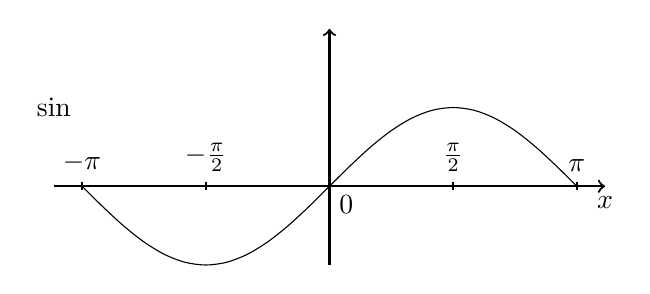
\begin{tikzpicture}[domain=-pi:pi]
\draw[->,thick] (-3.5,0) -- (3.5,0) node[below] {$x$};
\draw[->,thick] (0,-1) -- (0,2);
\node at (0,0) [below right] {$0$};
\node at (-3.5,1) {$\sin$};

\foreach \x/\y in {-pi/-\pi,-1.570/-\frac{\pi}{2},1.570/\frac{\pi}{2},pi/\pi}
	\draw[thick] (\x,-0.05) -- (\x,0.05) node[above] {$\y$};

\draw plot[smooth] (\x,{sin(\x r)});
\end{tikzpicture}

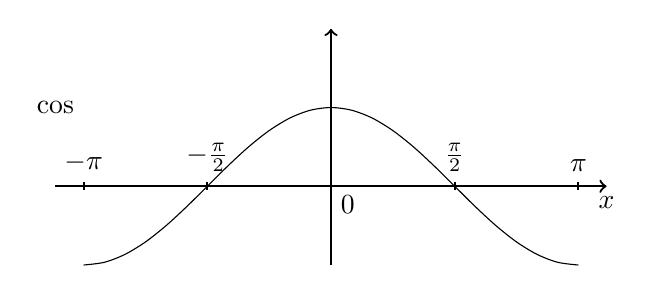
\begin{tikzpicture}[domain=-pi:pi]
\draw[->,thick] (-3.5,0) -- (3.5,0) node[below] {$x$};
\draw[->,thick] (0,-1) -- (0,2);
\node at (0,0) [below right] {$0$};
\node at (-3.5,1) {$\cos$};

\foreach \x/\y in {-pi/-\pi,-1.570/-\frac{\pi}{2},1.570/\frac{\pi}{2},pi/\pi}
	\draw[thick] (\x,-0.05) -- (\x,0.05) node[above] {$\y$};

\draw plot[smooth] (\x,{cos(\x r)});
\end{tikzpicture}

\begin{tikzpicture}
\draw[->,thick] (-3.5,0) -- (3.5,0) node[below] {$x$};
\draw[->,thick] (0,-1) -- (0,2);
\node at (0,0) [below right] {$0$};
\node at (-3.5,1) {$\tan$};

\foreach \x/\y in {-pi/-\pi,-1.570/-\frac{\pi}{2},1.570/\frac{\pi}{2},pi/\pi}
	\draw[thick] (\x,-0.05) -- (\x,0.05) node[above] {$\y$};

\draw plot[domain=0:1.2,smooth] (\x,{tan(\x r)});  \draw plot[domain=-1.2:0,smooth] (\x,{-tan(-\x r)});
\end{tikzpicture}
\Img{MA-16.04.2009-IMG-2}
\end{center}
\end{fdefinition}

\begin{fsatz}[Eigenschaften der trigonometrischen Funktionen]
\mbox{}\par
\begin{enumerate}[label=\roman*)]
\item $\cosx{0} = 1, \sinx{0} = 0$
\item $\cosx{-x} = \cosx{x}$ gerade Funktion\\
		$\sinx{-x} = -\sinx{x}$ ungerade Funktion

\item $\cosx{x + y} = \cosx{x} \mal \cosx{y} - \sinx{x} \mal \sinx{y}$\\
		$\sinx{x + y} = \sinx{x} \mal \cosx{y} + \cosx{x} \mal \sinx{y}$

\item $\cosx{x - y} = \cosx{x} \mal \cosx{y} + \sinx{x} \mal \sinx{y}$\\
		$\sinx{x - y} = \sinx{x} \mal \cosx{y} - \cosx{x} \mal \sinx{y}$

\item $\cosx{x} \mal \cosx{y} = \frac{1}{2} \rkl{\cosx{x + y} + \cosx{x - y}}$\\
		$\sinx{x} \mal \sinx{y} = \frac{1}{2} \rkl{\cosx{x - y} - \cosx{x + y}}$\\
		$\sinx{x} \mal \cosx{y} = \frac{1}{2} \rkl{\sinx{x + y} + \sinx{x - y}}$

\item $\cosx{2x} = \cos^2(x) - \sin^2(x)$\\
		$\sinx{2x} = 2 \sinx{x} \mal \cosx{x}$

\item $\cos^2(x) + \sin^2(x) = 1$\\
		$-1 \klgl \sinx{x}, \cosx{x} \klgl 1$

\item F�r alle $k \in \Z$ gilt:
		\[\left.\begin{array}{l}
		\cosx{x + 2\pi k} = \cosx{x}\\
		\sinx{x + 2\pi k} = \sinx{x}
		\end{array}\right\} 2 \pi\tx{-periodisch}\]
		\[\cosx{(2k + 1) \mal \frac{\pi}{2}} = 0\]
		\[\cosx{k \mal \pi} = (-1)^k\]
		\[\sinx{k \mal \pi} = 0\]
		\[\sinx{(2 \mal k + 1) \mal \frac{\pi}{2}} = (-1)^k\]
%TODO: Align to left
\end{enumerate}
\end{fsatz}

\section{Aufgabe 2.6}
\label{sec:Potenzreihen_und_elementare_Funktionen_A2_6}
Zu zeigen: $\cos^2(x) + \sin^2(x) = 1$ (Verwenden Summendarstellung von $\sin$, $\cos$ und Cauchy-Produkt)

L�sung siehe \vref{sec:Potenzreihen_und_elementare_Funktionen_A2_6L}.

\begin{bemerkung}
\mbox{}\par
\begin{enumerate}
\item Die Zahl $\pi$ kann man als das doppelte der ersten positiven Nullstelle vom Cosinus definieren.
		\begin{figure}[h]
		\centering
		\begin{tikzpicture}
		\draw (0,0) circle (2cm);
		\node[regular polygon, regular polygon sides=6, minimum size=4cm, draw] at (0,0) {};
		\end{tikzpicture}
		\Img{IMG-MA-09-04-21-1}
		\end{figure}
		Diese verwendet man zur einfacheren Berechnung (einfacher als �ber den Umfang von Vielecken) von $\pi$.

\item Eulersche Beziehung: $i = \sqrt{-1}$, $x \in \R$
		\begin{align*}
		e^{(ix)} &= \sum_{n = 0}^{\infty} \frac{(ix)^n}{n!} = \sum_{n = 0}^{\infty} \frac{(ix)^{2n}}{(2n)!} + \sum_{n = 0}^{\infty} \frac{(ix)^{2n + 1}}{(2n + 1)!}\\
		&= \sum_{n = 0}^{\infty} (i)^{2n} \frac{x^{2n}}{(2n)!} + \sum_{n = 0}^{\infty} i \mal \ub{(i)^{2n}}{= (-1)^n} \frac{x^{2n + 1}}{(2n + 1)!}\\
		&= \sum_{n = 0}^{\infty} (-1)^n \frac{x^{2n}}{(2n)!} + i \sum_{n = 0}^{\infty} (-1)^n \mal \frac{x^{2n + 1}}{(2n + 1)!}\\
		&= \cosx{x} + i \mal \sinx{x}
		\end{align*}
		\begin{figure}[h]
		\centering
		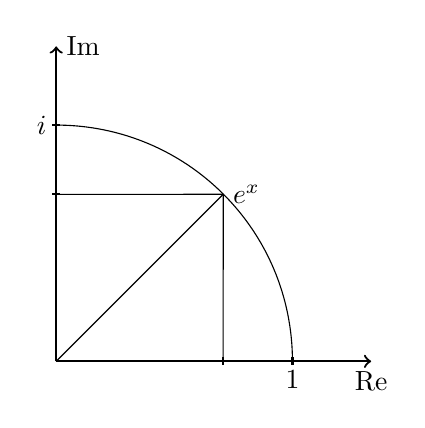
\begin{tikzpicture}
		\draw[->, thick] (0,0) -- (4.0,0) node[below] {Re};
		\draw[->, thick] (0,0) -- (0,4.0) node[right] {Im};
		\draw[in=0,out=90] (3,0) node[below] {$1$} to (0,3) node[left] {$i$};
		\draw (0,0) -- (45:3) node[right] {$e^x$};
		\draw (45:3) -- (2.12,0);
		\draw (45:3) -- (0,2.12);
		\node[below] at (1.06,0) {$\cosx{}$};
		\node[left] at (0,1.06) {$\sinx{}$};
		\draw[thick] (2.12,0.05) -- (2.12,-0.05);
		\draw[thick] (0.05,2.12) -- (-0.05,2.12);
		\draw[thick] (3,0.05) -- (3,-0.05);
		\draw[thick] (0.05,3) -- (-0.05,3);
		\end{tikzpicture}
		\end{figure}
		\Img{IMG-MA-09-04-21-2}

		$z = x + iy$ $x,y \in \R$\\
		$\overline{z} = x - iy$
		\Solved[Ist $\overline{z}$]{Herausfinden ob es $\overline{z}$ oder nur $z$ ist}

\item $\frac{1}{2} \rkl{e^{ix} + e^{-ix}}$
		\begin{align*}
		= &\frac{1}{2} \rklamm{\cosx{x} + i \mal \sinx{x} + \rklamm{\cosx{-x} + i \mal \sinx{-x}}}\\
		= &\frac{1}{2} \rklamm{\cosx{x} + i \mal \sinx{x} + \rklamm{\cosx{x} - i \mal \sinx{x}}}\\
		= &\cosx{x}\\
		&\frac{1}{2} \rkl{e^{ix} - e^{-ix}} = \dots = \sinx{x}
		\end{align*}
\end{enumerate}

\section{L�sungen}
\subsection{Aufgabe 2.5}
\label{sec:Potenzreihen_und_elementare_Funktionen_A2_5L}
L�sung zu Aufgabe \vref{sec:Potenzreihen_und_elementare_Funktionen_A2_5}.

\begin{enumerate}[label=\alph*)]
\item $\sum_{n = 0}^{\infty} 3n (x + 1)^n$
		\[\sum_{n = 0}^{\infty} 3n (x + 1)^n = \sum_{n = 0}^{\infty} \ub{3n}{a_n} (x - \ub{(-1)}{x_0})^n\]
		Entwicklungspunkt $x_0 = -1$\\
		Wurzelmethode
		\begin{align*}
		\lim_{n \ra \infty} \sqrt[n]{\betrag{a_n}} &= \lim_{n \ra \infty} \sqrt[n]{3n} = \lim_{n \ra \infty} \sqrt[n]{3} \mal \sqrt[n]{n}\\
		&= \lim_{n \ra \infty} \sqrt[n]{3} \mal \lim_{n \ra \infty} \sqrt[n]{n} = 1 \mal 1 = 1
		\end{align*}
		Konvergenzradius $r = 1$
		$(x_0 -r , x_0 + r) = (-2, 0) \subseteq K \subseteq \eklamm{-2, 0}$
		\begin{description}
		\item[$x = -2$] $\sum_{n = 0}^{\infty} 3n (-1)^n$ divergent nach Kriterium
		\item[$x = 0$] $\sum_{n = 0}^{\infty} 3n \mal (1)^n (\lim_{n \ra \infty} 3_n = \infty \neq 0)$ nach dem notwendigen Kriterium divergent
		\end{description}
		\Ra $K = (-2, 0)$

\item $\sum_{n = 0}^{\infty} \frac{1}{n^n} \mal x^n$
		\[\sum_{n = 0}^{\infty} \frac{1}{n^n} \mal x^n = \sum_{n = 0}^{\infty} \ub{\frac{1}{n^n}}{= a_n} \mal (x - \ub{0}{x_0})^n\]
		Entwicklungspunkt $x_0 = 0$\\
		Wurzelmethode
		\[w = \lim_{n \ra \infty} \sqrt[n]{\betrag{a_n}} = \lim_{n \ra \infty} \sqrt[n]{\frac{1}{n^n}} = \lim_{n \ra \infty} \frac{1}{n} = 0\]
		Konvergenzradius $r = \infty$
		\Ra Konvergenzbereich $K = \mb{R}$

\item $\sum_{k = 0}^{\infty} \frac{(2x + 1)^k}{k + 3}$
		\[\sum_{k = 0}^{\infty} \frac{(2x + 1)^k}{k + 3} = \sum_{k = 0}^{\infty} \frac{1}{k + 3} \rkl{2 \rkl{x - \rkl{- \frac{1}{2}}}}^k = \sum_{k = 0}^{\infty} \ub{\frac{2^k}{k + 3}}{= a_k} \rkl{x - \rkl{-\frac{1}{2}}}^k\]
		Entwicklungspunkt $x_0 = -\frac{1}{2}$
		Quotientenmethode
		\begin{align*}
		q &= \lim_{k \ra \infty} \betrag{\frac{a_k}{a_{k + 1}}} = \lim_{k \ra \infty} \frac{2^k}{k + 3} \mal \frac{(k + 4)}{2^{k + 1}} = \lim_{k \ra \infty} \frac{k + 3}{2(k + 4)}\\
		&= \frac{1}{2} \lim_{k \ra \infty} \frac{1 + \frac{3}{k}}{1 + \frac{4}{k}} = \frac{1}{2}\\
		&\Ra r = q \frac{1}{2}
		\end{align*}
		$(-1, 0) \subseteq K \subseteq \eklamm{-1, 0} \Ra K = \eklamm{-1, 0}$
\end{enumerate}

\subsection{Aufgabe 2.6}
\label{sec:Potenzreihen_und_elementare_Funktionen_A2_6L}
L�sung zu Aufgabe \vref{sec:Potenzreihen_und_elementare_Funktionen_A2_6}.

\begin{align*}
\sin^2(x) &= \rklamm{\sum_{k = 0}^{\infty} \ub{(-1)^k \mal \frac{x^{2k + 1}}{(2k + 1)!}}{= A_k}} \mal \rklamm{\sum_{k = 0}^{\infty} \ub{(-1)^k \mal \frac{2^{2k + 1}}{(2k + 1)!}}{= B_k}}\\
&\stack{\tx{CP}}{=} \sum_{k = 0}^{\infty} \rklamm{\sum_{l = 0}^{k} A_l \mal B_{k - l}} = \sum_{k = 0}^{\infty} \rklamm{\sum_{l = 0}^{\infty} (-1)^l \frac{x^{2l + 1}}{(2 l + 1)!} \mal (-1)^{k - l} \mal \frac{x^{2 (k - l) + 1}}{(2 (k - l) + 1)!}}\\
&= \sum_{k = 0}^{\infty} (-1)^k x^{2k + 2} \textcolor{blue}{\frac{1}{(2k + 2)!}} \sum_{l = 0}^{k} \ub{\frac{\textcolor{blue}{(2k + 2)!}}{(2l + 1)! \mal (2k - 2l + 1)}}{\binom{2k + 2}{2l + 1}}\\
&= \sum_{k = 0}^{\infty} (-1)^k \mal \frac{x^{2k + 2}}{(2k + 2)!} \mal \frac{2^{2k + 2}}{2}\\
&= \sum_{n = 0}^{\infty} (-1)^n \frac{x^{2n}}{(2n)!} \mal 2^{2n - 1}
\end{align*}

\begin{align*}
\cos^2(x) &= \rklamm{\sum_{n = 0}^{\infty} \ub{\rklamm{-1}^n \mal \frac{x^{2n}}{(2n)!}}{= A_n}} \mal \rkl{\sum_{n = 0}^{\infty} \ub{(-1)^n \mal \frac{x^{2n}}{(2n)!}}{= B_n}}\\
&\stack{\tx{CP}}{=} \sum_{n = 0}^{\infty} \mal \sum_{l = 0}^{n} A_l \mal B_{n - l}\\
&= \sum_{n = 0}^{\infty} \sum_{l = 0}^{n} (-1)^l \mal \frac{x^{2l}}{(2l)!} \mal (-1)^{n - l} \mal \frac{x^{2 (n - l)}}{(2 (n - l))!}\\
&= \sum_{n = 0}^{\un} (-1)^n \frac{x^{2n}}{(2n)!} \sum_{l = 0}^{n} \ub{\frac{(2n)!}{(2l)! \mal (2n - 2l)!}}{= \binom{2n}{2l}}\\
&= \rklamm{\sum_{n = 1}^{\un} (-1)^n \frac{x^{2n}}{(2n)!} \mal 2^{2n - 1}} + 1
\Ra & \sin^2(x) + \cos^2(x) = 1
\end{align*}
\end{bemerkung}
